% --- SLIDE 7: CONCEPT DEVELOPMENT (STRUTTURA) ---
\begin{frame}{Concept Development: Components and Materials}
    
    \vspace{0.4cm}
    
    % Le tre colonne allineate in alto (opzione [T])
    \begin{columns}[T]
        
        % --- 1. ELASTIC COMPONENT ---
        \begin{column}{0.31\textwidth}
            \centering
            % INSERISCI QUI LA TUA PRIMA FOTO
            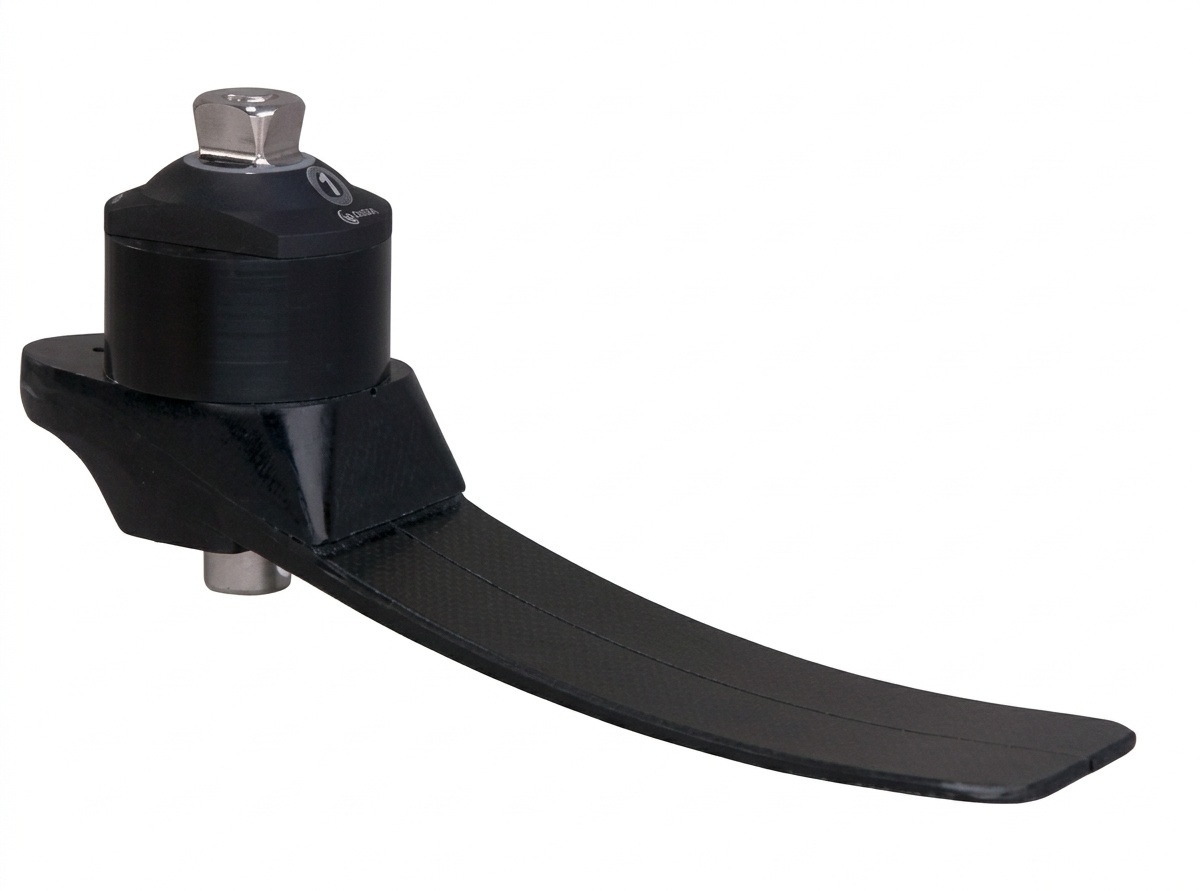
\includegraphics[width=0.95\linewidth]{image/foto_lamina.png} 
            
            \vspace{0.3cm}
            \begin{block}{1. Elastic Component}
                \scriptsize \textbf{ESR Carbon Fiber Blade:} Acts as the main tendon. Manages the \textit{Toe-off} phase and stores propulsive energy.
            \end{block}
        \end{column}
        
        % --- 2. STRUCTURAL MATRIX ---
        \begin{column}{0.34\textwidth}
            \centering
            % INSERISCI QUI LA TUA SECONDA FOTO
            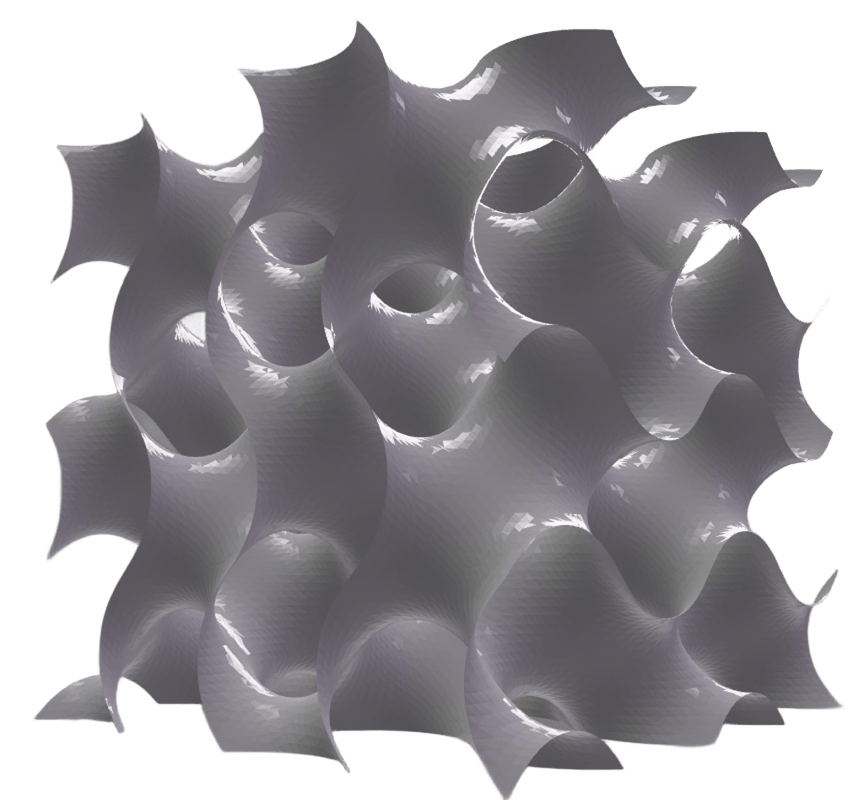
\includegraphics[width=0.87\linewidth]{image/Gyroid.png} 
            
            \vspace{0.08cm}
            \begin{block}{2. Structural Matrix}
                \scriptsize \textbf{Dermal Layer (TPMS):} Flexible TPU scaffold with gyroid structure. Sustains the baseline load and guides the spatial deformation.
            \end{block}
        \end{column}
        
        % --- 3. INTELLIGENT CORE ---
        \begin{column}{0.31\textwidth}
            \centering
            % INSERISCI QUI LA TUA TERZA FOTO
            \vspace{0.45cm}
            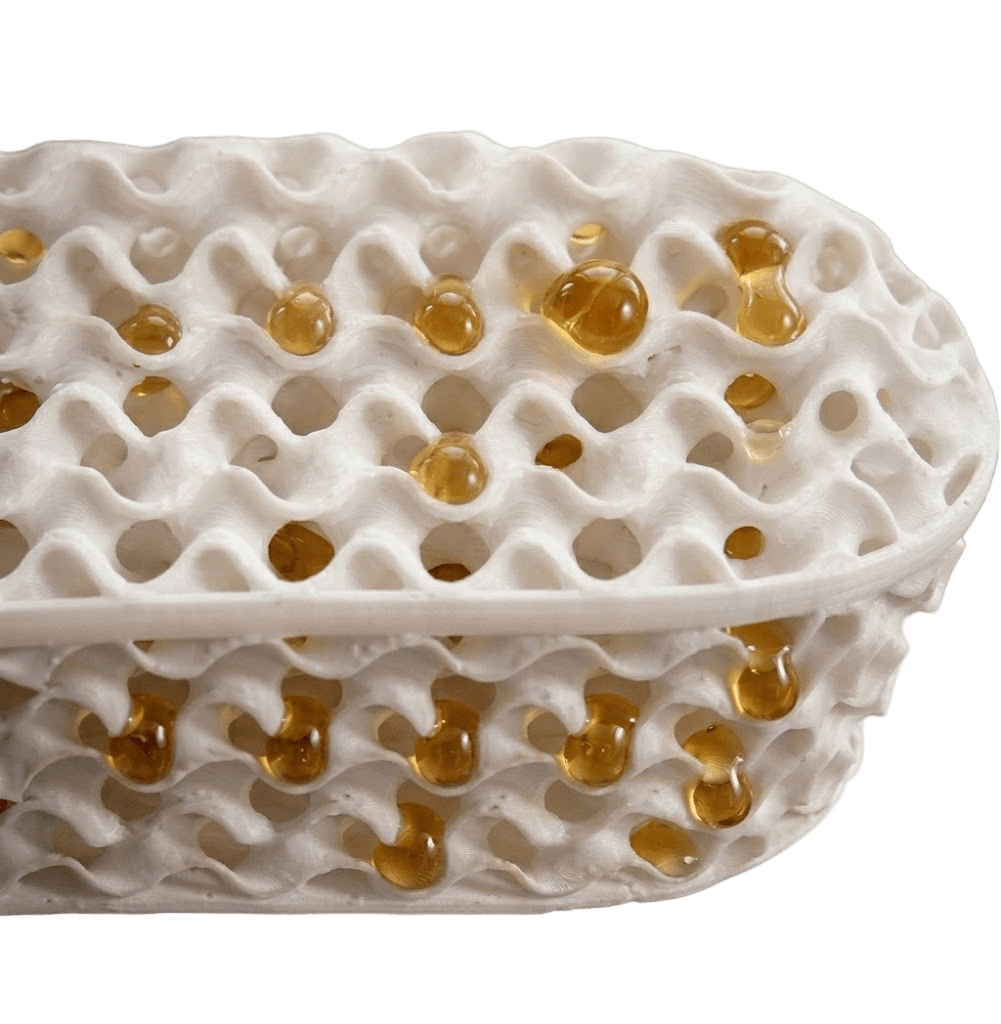
\includegraphics[width=0.95\linewidth]{image/foto_stf.png} 
            
            \vspace{-0.35cm}
            \begin{block}{3. Intelligent Core}
                \scriptsize \textbf{Adipose Tissue (STF):} Confined non-Newtonian fluid (suspension of $SiO_2$ nanoparticles in PEG). Modulates stiffness based on impact velocity.
            \end{block}
        \end{column}
        
    \end{columns}
\end{frame}